\subsection{Simulating neural activity in a neural population} \label{sec:results:simulations}

To test the described method for inferring functional connectivity from calcium imaging data, we simulated networks (according to our model, Eqs. \ref{eqn:glm:definition} -- \ref{eqn:F:definition}) of stochastically connected neurons.  Although simulations ran at $1$ msec time discretization, imaging rate was assumed to be much slower. Simulations lasted anywhere between 5 minutes and 1 hours (of simulated time).  Model parameters were chosen based on experimental data available from the literature \cite{Braitenberg1998,Urquijo2000,Lefort2009,Sayer1990}.

More specifically, the network was divided into excitatory (80\%) and inhibitory (20\%) neurons \cite{Braitenberg1998,Urquijo2000}, each respecting Dale's law, i.e., each neurons was either excitatory or inhibitory (corresponding to all positive or all negative columns in our functional connection weight matrix, $\bw$). Neurons were randomly connected to each other with probability $0.1$ \cite{Braitenberg1998,Lefort2009}.  Synaptic weights for excitatory connections, as defined by EPSP peak amplitude, were randomly drawn from exponential distribution with the mean of $0.5 \mu V$ \cite{Lefort2009,Sayer1990}. To convert these into functional connectivity weights, we note that $w_{ij}=1$ corresponds to a jump in $J_i=1$, immediately following a spike from neuron $j$.  Defining $V_\delta$ as the difference between threshold and rest for a neuron, and $V_E$ as the peak amplitude of an EPSP (and similarly for IPSP's), we can say the change in probability after a spike is $\Delta P=V_E/V_\delta$. Because Eq. \ref{eqn:glm:definition} provides the same quantity in our model parameter, $w_{ij}$, we have:

\begin{equation}\label{eqn:convert}
\w_{ij}=\ln(-\ln(e^{-r_i\tau_w}-V_E/V_{\delta})/r_i\tau_w),
\end{equation}

\noindent where $r_i=\exp(b_i)$ is the base firing rate of neuron $i$ and $\tau_w=10$ msec was the typical EPSP/IPSP scale over which single EPSP affects the firing probability of the neuron $i$ \cite{}. Inhibitory connections were also drawn from exponential distribution; their strengths chosen so as to balance excitatory and inhibitory currents in the network, and achieve an average firing rate of  $\approx 5 $ Hz \cite{Abeles01}. Practically, the mean strength of inhibitory connections was about 10 times larger than that of the excitatory connections. PSP shapes were modeled as an alpha function \cite{Koch99}, by differencing of two exponentials, corresponding to a sharp rise and relatively slow decay \cite{Sayer1990}.
%The time course of functional connectivity weights $\w_{ij}(t)$ was modeled as the difference of two exponentials, resulting in a rise time of $\tau_r=1$ msec and decay time of $\tau_{E_d}=10$ msec for excitatory and $\tau_{I_d}=20$ msec for inhibitory currents . In practice, we sampled time constants from uniform distributions with means as stated above and support of $\pm 25 \%$ of the means.
We neglected conduction delays, given that the time delay below $\sim 1$ msec expected in local cortical circuit was smaller than the time step of our computer simulation.  Each neuron also had an exponential refractory current with a $10$ msec time constant \cite{Koch99}. XXX Y: did that not get sampled from some distribution? XXX

Parameters for the calcium dynamics and observation statistics were chosen according to our experience with several cells analyzed using algorithm of \cite{Vogelstein2009}, and conformed to other experimental observations \cite{ImagingManual,HelmchenSakmann96,BrenowitzRegehr07}. Each parameter was generated from a normal distribution with specified mean and variance at about 30\% of the mean, truncated at the lower bound at about 30\% of the mean value.  Table \ref{table:caparm} provides details for each of the parameters in our model.

\begin{table}[h!b!p!]
\caption{Table of simulation parameters. $\mathcal{E}(\lambda)$ indicates an exponential distribution with $\lambda$, and $\mathcal{N}(\mu,\sigma^2)$ indicates a truncated normal with mean $\mu$ and variance $\sigma^2$, and lower bound of one standard deviation below the mean.}\label{table:caparm}

\begin{tabular}{lll}
\hline
Total neurons & 10-500 \\
Excitatory neurons & $80\%$ \\
Connections sparseness & $10\%$ \\
Baseline firing rate & $5$  & Hz\\
\hline
EPSP peak height 	& $\sim \mathcal{E}(0.5)$ 	& $\mu$V \\
IPSP peak height 	& $\sim -\mathcal{E}(2.3)$ 	& $\mu$V \\
EPSP rise time 		& $\sim \mathcal{N}(1,0.3)$ & msec \\
EPSP decay time 	& $\sim \mathcal{N}(10,2.5)$& msec \\
IPSP rise time 		& $\sim \mathcal{N}(1,0.3)$ & msec \\
IPSP decay time 	& $\sim \mathcal{N}(20,7)$ 	& msec \\
\hline
Calcium std. $\sigma_c$ & $\sim \mathcal{N}(28,10)$ & $\mu$M \\
Calcium jump after spike, $A_c$ &  $\sim \mathcal{N}(80,20)$ & $\mu$M \\
Calcium baseline, $C_b$ & $\sim \mathcal{N}(24,8)$ & $\mu$M \\
Calcium decay time, $\tau_c$ & $\sim \mathcal{N}(500, 170)$ & msec \\
Mean photon budget $\alpha_c$ & $1$--$80$ & Kph/neuron/frame \\
Dissociation constant, $K_d$ & $200$ & $\mu$M \\
\hline
\end{tabular}
\end{table}


\subsection{Inferring functional connectivity from the simulated calcium imaging data} \label{sec:results:inference}

With neural population activity prepared as described in the previous section, we used our inference algorithms to reconstruct the functional connectivity matrix from simulated fluorescence data. Specifically, we estimated the connectivity matrix by maximizing $E[\ln P[n_i(t)| \bh(t); b_i, \bw_i]]$ with respect to $\{b_i,\bw_i\}$, for each neuron (c.f. Eq. \ref{eqn:loglik:definition-expl}), using both the embedded-chain-within-blockwise-Gibbs approach as well as using factorized approximation, Figure \ref{fig:scatters}.  We found that factorized approximation algorithm was able to provide reconstructions almost as accurate as the exact embedded-chain-within-blockwise-Gibbs approach --- $r^2=0.47$ versus $r^2=0.48$ --- when parameters corresponded to a realistic (but relatively high quality) preparation, given $10$ minutes simulation time, in a population of $N=25$ neurons. Figure \ref{fig:example_traces} depicts a couple different fluorescence traces, of varying SNR. 
factorized
\begin{figure}[h]
\centering
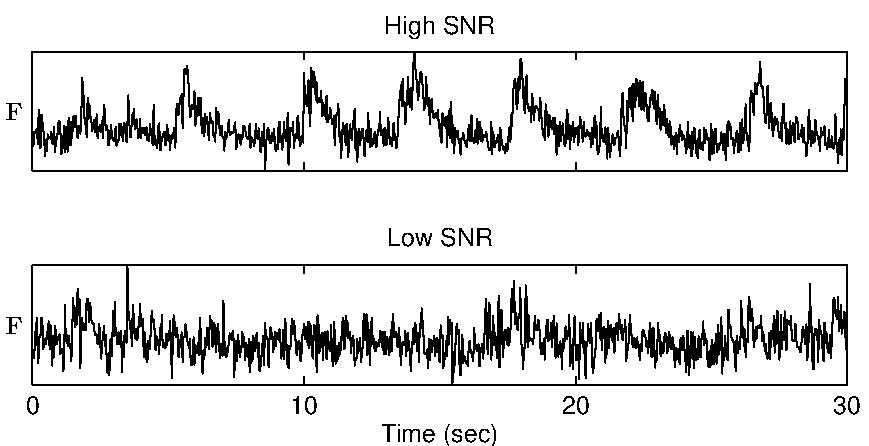
\includegraphics[width=\hsize]{../figs/example_traces}
\caption{Two in vivo fluorescence traces (top) and their corresponding inferred spike trains (bottom).  The left panels show a high SNR case, that is sufficient quality for the factorized approximation to work nearly as well as the embedded-chain-within-Gibbs approach.  The right panels show a low SNR case, in which the factorized approach is insufficient. The ordinate is in arbitrary units.  Data from the laboratory of Tom Mrsic-Flogel.}
\label{fig:example_traces}
\end{figure}

To compare the quality of our inferences using only the fluorescence traces, we also estimated the weights using the true spike trains, down-sampled to the frame rates of calcium imaging.  Indeed, the quality of our estimates using the fluorescence traces are worse than those obtained from the down-sampled spike trains; $r^2=0.57$ using the down-sampled spike trains.  Note that $r^2\rightarrow 1$ as $T \rightarrow \infty$, when using the true (i.e., not down-sampled) spike trains, as guaranteed by our model.  Indeed, when using the true spike trains, $r^2=XXX$ for this simulation.  This suggests that as imaging rates increase, we can expect a corresponding increase in accuracy of our functional connectivity weight estimates.

%Fluorescence data is generally acquired at low frame rate and, so, one of its main limitations is bad time-resolution of the observed spike trains. To determine the impact of this constraint on the connectivity reconstructions, and, thus, to determine how close calcium imaging may approach reconstructions from spike trains directly observed under comparable conditions, we conducted this experiment. We observed that at intermediate SNR reconstructions from calcium imaging closely resembled such obtained directly from spike trains, and at higher SNR reconstruction with the quality same with original spike trains was achieved, Figure \ref{fig:scatters} and \ref{fig:recvar-SNR}.


%\begin{align}
% \label{eqn:likelihoodGLMmoda}
% &E[\ln P[n_i(t)| \bh(t); b_i, k_i, \bw_i, S(t)]
% 	=\sum_t \left( n_i(t) \ln J_i(t) - (1-n_i(t)) \exp(J_i(t)) \Delta \right), \\
% \label{eqn:likelihoodGLMmodb}&J_i(t)=b_i+\sum\limits_j \sum\limits_{t'<t} \w_{ij}(t-t')n_{j}(t')=
% b_i+\sum\limits_j w_{ij} h_j(t).
% \end{align}

\comment{The sum in Eqs.\ref{eqn:likelihoodGLMmoda} and \ref{eqn:likelihoodGLMmodb} was over the sample of $\{n_i(t)\}$, produced with our spike sampling algorithm, discretized over the time-bins $t'$ with the width corresponding to the calcium imaging frame rate (i.e. 30 ms for 33 Hz and 15 ms for 66 Hz). In one of the two cases we considered, EPSP time-profiles were assumed to be ``known'' exponential, and the weights were estimated using reduced histories $h_{i}(t)=\sum_{t'<t} \exp(-(t-t')/\tau_h)n_{i}(t')$ with the time constant $\tau_h=10$ ms (i.e. second equation in Eq. \ref{eqn:likelihoodGLMmodb}). In the second case we considered, the time dependence of $\w_{ij}(t)$ was assumed to be unknown and the first equation in Eq. \ref{eqn:likelihoodGLMmodb}) was used to correlate $n_i(t)$ with $n_j(t')$ for $t'<t$ up to a given depth $m$.  In this latter case, since each next term in Eq. \ref{eqn:likelihoodGLMmodb}) was significantly smaller than the previous one, we found that the best results were obtained if we took $m=1$ (i.e. minimizing number of unknown variables given certain amount of data).
In either case, we described the connection weight between two neurons by a scalar quantity $w_{ij}^s=\text{sign}(\w_{ij})\max_{t} |\w_{ij}(t)|$, which thereafter was used to compare true and reconstructed connectivity weights in all examples below.}

\begin{figure}[h]
\centering
\begin{minipage}[c]{0.45\hsize}
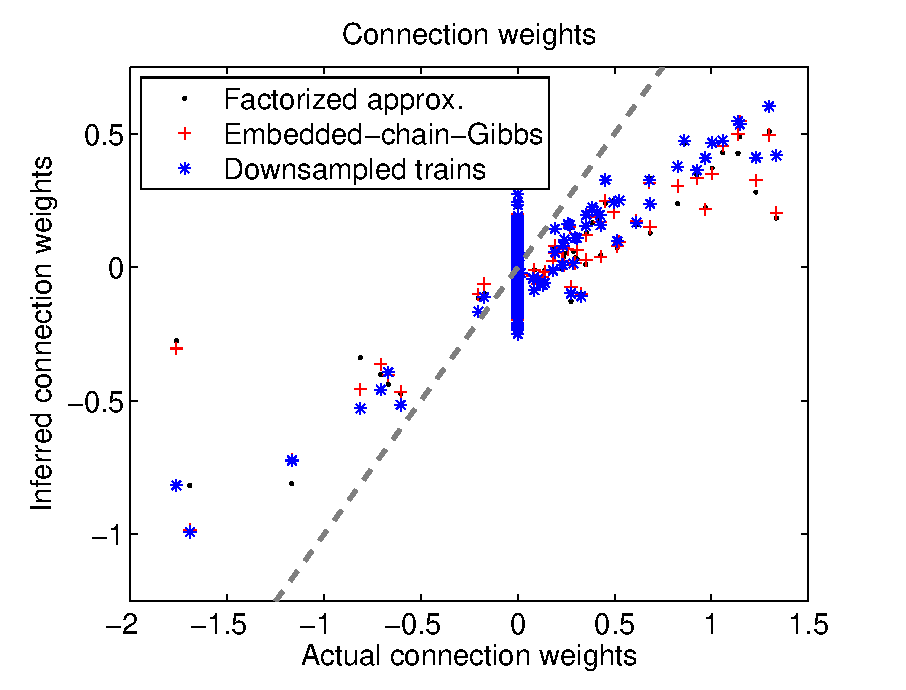
\includegraphics[width=\hsize]{../figs/FigureA3_scatter_three}
\end{minipage}
\begin{minipage}[c]{0.45\hsize}
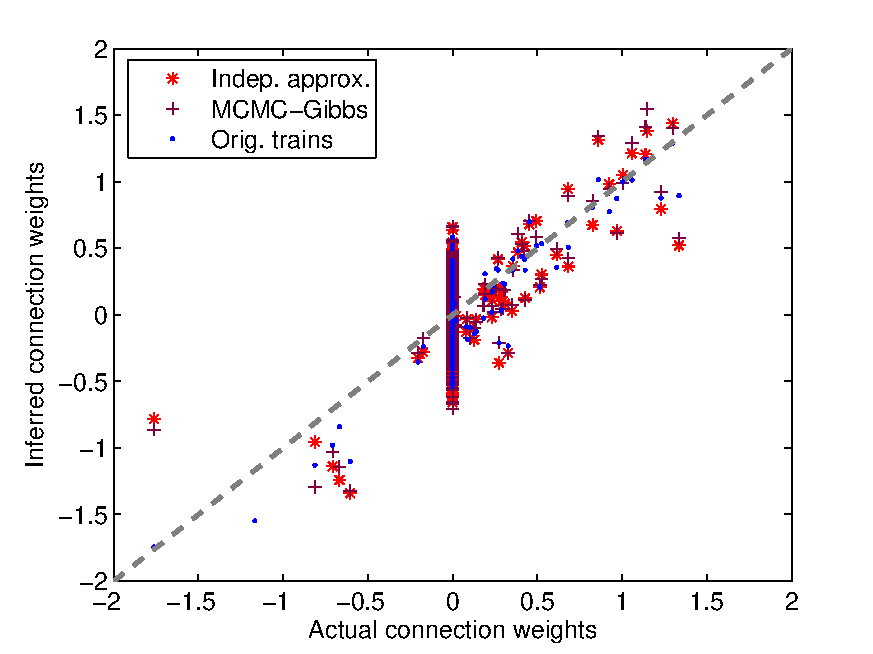
\includegraphics[width=\hsize]{../figs/FigureA3_scatter_three_corrected}
\end{minipage}
\caption{Functional connectivity matrix can be reconstructed from calcium imaging data. In the upper panels inferred connection weights are shown in a scatter plot versus real connection weights, with inference performed using factorized approximation algorithm, exact embedded-chain-within-blockwise-Gibbs approach, and original spike trains observed at the frame rate of the calcium imaging. Network of $N=25$ neurons was used, firing at $\approx 5$ Hz, and imaged for T=600 sec at intermediate SNR (photon budget 10Kph/neuron/frame, see below). $r^2=0.47$ for factorized approximation algorithm was found, $r^2=0.48$ for embedded-chain-within-blockwise-Gibbs approach, and $r^2=0.57$ for the original spike trains. Thus, factorized approximation produced results almost as accurate as the exact embedded-chain-within-blockwise-Gibbs approach, and almost as accurate as the original spikes. Inferred connectivity weights (upper left) were scaled with respect to true connectivity by a constant amount due to time discretization bias (see below); other than scale, inferred connectivity represented the true connectivity matrix very well (upper right). Thus, calcium imaging is sufficient to identify connected pairs of neurons reliably.} \label{fig:scatters} \end{figure}

\subsection{Scale bias in inferred connection weights due to coarse time discretization of calcium imaging data}

That all three approaches considered in Figure \ref{fig:scatters} exhibit a significant scaling bias suggests that down-sampling spike times introduces this bias.  We conjectured that this is caused by the discrepancy between $\Delta \approx 15-30$ msec and the assumed PSP time scale $\approx 10-20$ msec. Properly estimating the magnitude of the connection weights $w_{ij}$ is based on empirically evaluating the spike-triggered probability of neuron $i$ to fire, conditioned on neuron $j$. Note that most triggered spikes of neuron $i$ will occur within $\approx 10-20$ msec from a triggering spike of neuron $j$ (because of our assumed values for $\tau_w$). However, when spike trains are discretized into large time-bins, e.g. $\Delta = 30$ msec, a significant fraction of such triggered spike pairs seem coincident, as opposed to causal (because both the triggering and triggered spikes end up in the same time-bin). Therefore, we empirically observe a smaller number of triggered spikes than occur, causing a scale bias in $w_{ij}$.

To quantitatively estimate the magnitude of this scale bias and correct it, consider two neurons coupled with small weight $w_{12}$. Assume that, aside from this coupling, these neurons fire with baseline firing rate of $r=f(b)=\exp(b)$, $b \gg w_{12}$. In order to estimate $w_{12}$ we observe the number of spike pairs such that the first neuron fired after the second neuron over some small period of time $\tau_w \ll t' \ll 1/r$, which is in excess of the baseline firing rate $\Delta n(2\rightarrow 1) = n(2\rightarrow 1) - r t' \approx f'(b) \int  w_{12} \exp(-t/\tau_w)$ dt.

Now, assume that spike trains were additionally discretized into time-bins of size $\Delta$, and only the spikes that occurred in different time-bins $t'<t$ were considered as non-coincidental. In this case, the number of spike pairs such that the spike of the first neuron followed that of the second neuron observed empirically is: 

\begin{equation}
\Delta n'(2\rightarrow 1) \approx f'(b) \int\limits_0^\Delta \frac{1}{\Delta} \int\limits_{\Delta}^T \exp(-(t_2-t_1)/\tau_w) \text{dt}_1 \text{dt}_2.
\end{equation} 

The ratio of this empirical count, $\Delta n'(2\rightarrow 1)$, to that expected from our model for given $w_{12}$, $\Delta n(2\rightarrow 1)$, is the theoretical scale bias:

\begin{equation}\label{eqn:bias}
\Delta n'_{12}/\Delta n_{12}\approx \frac{1-\exp(-\Delta/\tau_w)}{\Delta/\tau_w}.
\end{equation}

In Figure \ref{fig:bias} we plotted this estimated magnitude versus that empirically observed from our simulations for different values of $\Delta$. As can be seen from Figure \ref{fig:bias}, simple theoretical estimate Eq. \ref{eqn:bias} describes observed scale bias quite well.  This scale bias could potentially be overcome by inferring spike trains using the superresolution feature of \cite{VogPan09}, i.e., sampling spikes with a finer temporal resolution than the image rate.

\begin{figure}[h]
\centering
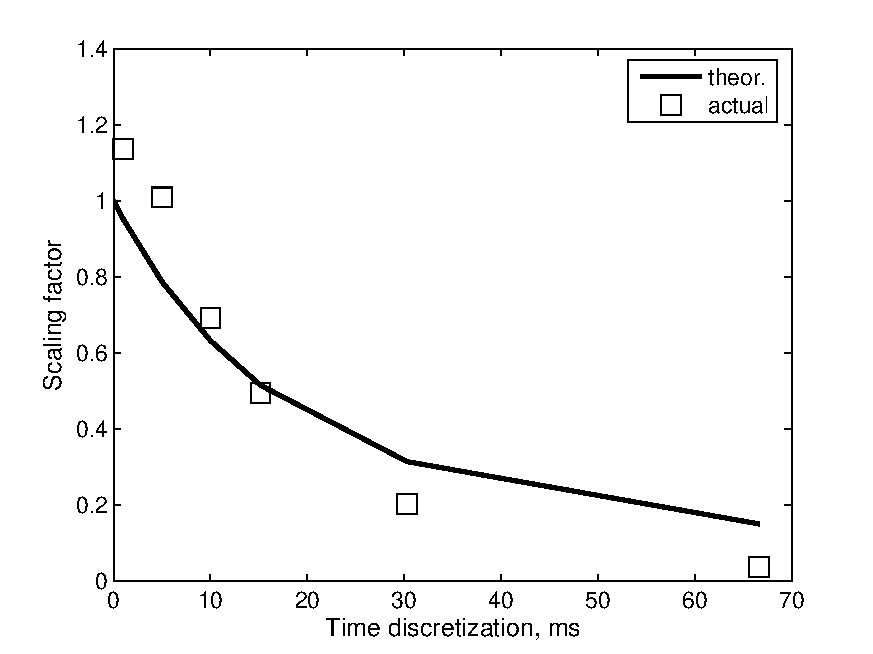
\includegraphics[width=3in]{../figs/FigureA4_scale_bias}
\caption{The low-frame rate of calcium imaging can explain the observed scale bias from Figure \ref{fig:scatters}.  Our theoretical scale bias is determined by considering what fraction of spikes would fall within a single image frame, which is a function of $\Delta$ (c.f. Eq. \ref{eqn:bias}).  The center of each square indicates the mean scale bias of 5 simulations, the extent of each square indicates one standard deviation, and the errorbars indicate the $95$th and $5$th percentiles. XXX Y: can you correct these details? XXX}
\label{fig:bias}
\end{figure}


\subsection{Impact of different imaging frame rates, noise levels, and durations on the estimator accuracy}

\begin{figure}[h]
\centering
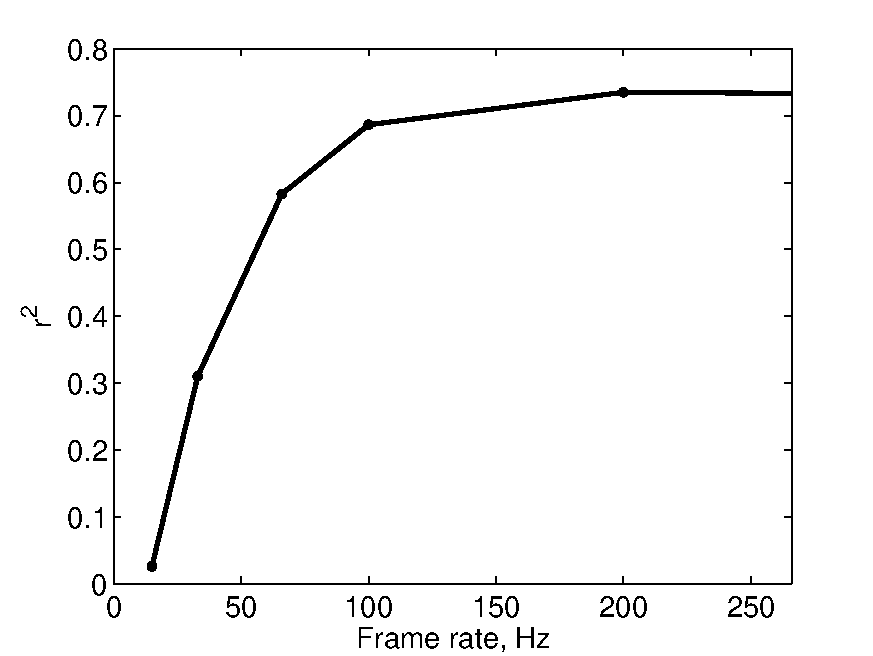
\includegraphics[width=3in]{../figs/FigureA5_recvar}
\caption{Accuracy of the inferred connectivity weights as function of the frame rate of calcium imaging. Connectivity matrix here was inferred from the original spike trains observed at corresponding frame rates, thus establishing the upper performance bound for inference using calcium imaging data. A network of $N=25$ neurons, firing at $\approx 5$ Hz and imaged for $T=600$ sec was used.}
\label{fig:recvar}
\end{figure}

\begin{figure}[h]
\centering
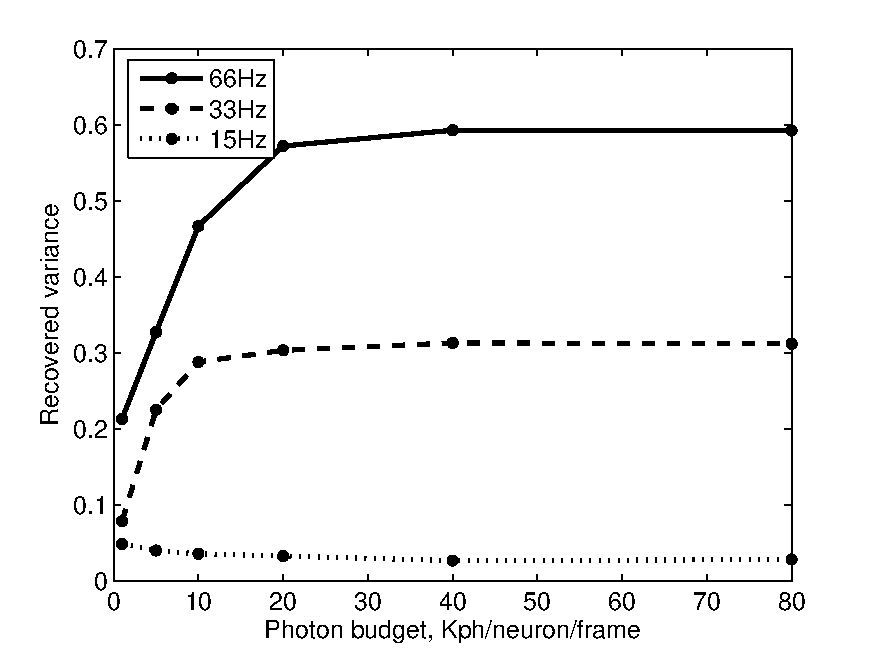
\includegraphics[width=3in]{../figs/FigureA6_recvar_SNR}
\caption{Accuracy of inferred connectivity weights as function of the noise amount in the calcium imaging data, as quantified by experimental photon budget per neuron-frame, for frame rates of 15 Hz, 33 Hz and 66 Hz. Photon counts on the order of 20-40 Kph/frame/neuron are required to achieve the upper bound due by the frame rate. Connectivity matrix here was inferred from simulated fluorescence data using factorized approximation algorithm. Simulation conditions are the same as in Figure \ref{fig:recvar}.  Vertical black lines indicate noise levels for the two example traces shown in Figure \ref{fig:example_traces}, as determined using the SMC approach to estimate $\theta_i$ as described in Section \ref{sec:methods:indep}.}
\label{fig:recvar-SNR}
\end{figure}

\begin{figure}[h]
\centering
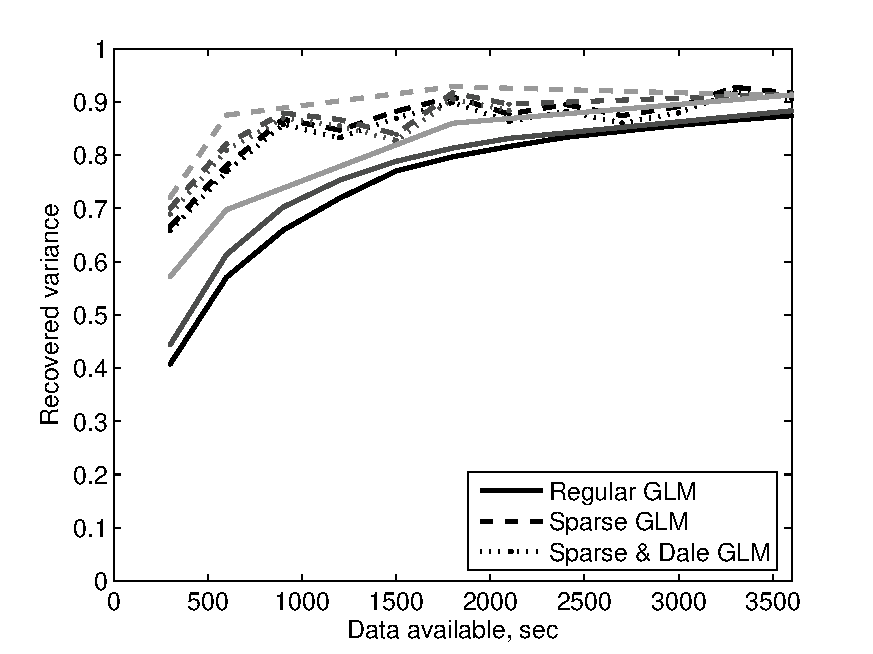
\includegraphics[width=3in]{../figs/FigureA7_recvar_NT}
\caption{Accuracy of inferred connectivity weights as function of the imaging time and neural population size. Incorporating simple priors such as exponential prior on the connectivity weights allows to boost reconstruction accuracy dramatically (dashed lines). In this latter case, $T=300$ sec is already sufficient to recover 70\% of the variance in the connection weights. Incorporating Dale's prior leads to only marginal improvement (dotted line). As shown in the methods, reconstruction accuracy does not depend on the neural population size $N$.
Here, neural population from $N=10$ to $N=200$ were simulated for different $T$, where
$N=200$ (gray) and $N=100$ (black) are shown. All networks were prepared in similar state by adjusting strength of inhibitory connections to achieve similar mean firing rate $\approx 5$ Hz, although actual firing rate in these networks could vary. In all cases, $T=5$ min - 0.5 hour is sufficient to produce accurate reconstructions.
}
\label{fig:recvar-NT}
\end{figure}


What minimal conditions for the experimental setup should be met to allow for successful reconstruction of the connectivity from calcium imaging data? In Figures \ref{fig:recvar} -- \ref{fig:recvar-NT} we address this question. Figure \ref{fig:recvar} shows the quality of the inferred connectivity matrix as function of the imaging frame rate; imaging frame rates 30-60 Hz are needed to achieve meaningful reconstruction results. These imaging frame rates are feasible for already existing experimental setups \cite{NguyenParker01,ReddySaggau05,Iyer06,SalomeBourdieu06,ReddySaggau08}. Figure \ref{fig:recvar-SNR} shows the quality of the inferred connectivity matrix as function of effective SNR and photon budget. Operationally, we define effective SNR here as $eSNR=$ XXX and photon budget as $1/\gamma$XXX. Note, therefore, that the relationship between $eSNR$ and $1/\gamma$ is XXX. From our experience with the analysis of real cells \cite{Vogelstein2009}, the eSNR in real data was $\sim XXX$ for in vivo data collected at 15  Hz and $\sim XXX$  for in vitro data at the same frame rate. As can be seen from Figure \ref{fig:recvar-SNR}, the effective SNR necessary for accurate reconstructions was $XXX$. For lower photon counts, the amount of noise in calcium imaging data degraded inferred connectivity matrices significantly. Finally, Figure \ref{fig:recvar-NT} shows the quality of the inferred connectivity matrix as function of the experimental duration. The minimal duration for a particular $r^2$ depended substantially on whether prior information about the distribution of connectivity weights was incorporated into the M-step (as described in detail below). In particular, for the M-step lacking a sparse prior, the calcium imaging duration necessary to achieve $r^2=0.5$ for the reconstructed connectivity matrix was $T\approx 10$ min, whereas, for the same data, when incorporating a sparse prior, $r^2>0.5$ was achieved already at $T\sim 5$ min. These numbers appear to be well within limitations of the existing experimental preparations. Furthermore, in agreement with theoretical analysis in Section \ref{sec:methods}, the accuracy of the reconstruction did not depend on the size of imaged neural population, with the same reconstruction quality observed for the same amount of data for $N=50-200$ neurons. In all cases, good reconstructions were obtained  with $T\sim 5$--$30$ min of calcium imaging data.


\subsection{Accuracy of the estimates and Fisher information matrix} \label{sec:methods:accuracy_Fisher}

XXX THIS SHOULD PROBABLY BE REDUCED A BIT XXX

To determine the necessary amount of data for accurate estimation of the functional connectivity matrix, we calculate Fisher information for $P[\bw| \bX]$. For clarity, we assume here that $\Delta \rightarrow 0$, and so $f(J)\approx e^J\Delta$, and that spike trains are known perfectly, thus there is no corruption due to inference from low-SNR calcium imaging data. We also assume that spikes couple only over a single time bin. Then, we write the Fisher information matrix as:

\begin{equation}
\begin{array}{rl}
C^{-1}=\left[\frac{\partial (-\ln P)}{\partial \w_{ij}\partial \w_{i'j'}}\right]
=-&\delta_{ii'}\sum\limits_t\left[
n_i(t)n_{j}(t-1)n_{j'}(t-1)\left(-\frac{f'(J_i(t))^2}{f(J_i(t))^2} +
\frac{f''(J_i(t))}{f(J_i(t))}\right) \right. \\
&\left.-(1-n_i(t))n_{j}(t-1)n_{j'}(t-1)f''(J_i(t))\right].
\end{array}
\end{equation}
 where $f'$ and $f''$ correspond to the first and the second derivatives of our linking function (c.f Eq. \ref{eqn:glm:definition}), and $\delta_{ii'}$ is 
 the Kronecker's delta symbol ($\delta_{ii'}=1$ for $i=i'$, and $\delta_{ii'}=0$ otherwise).  Letting $f(J)=e^J\Delta$, this may be rewritten as:

\begin{equation}\label{eqn:fisher}
\begin{array}{rl}
C^{-1}
&=\delta_{ii'} T P[n_i(t)=0, n_j(t-\Delta)=1, n_{j'}(t-\Delta)=1]E[e^{J_i(t)}|n_i(t)=0, n_j(t-\Delta)=1, n_{j'}(t-\Delta)=1] \\
&= T\left[(r \tau_w)\delta_{ii'}\delta_{jj'}+O((r \tau_w)^2)\right]r.
\end{array}
\end{equation}

\noindent where $ \tau_w$ is ``the coincidence time'' --- the typical EPSP/IPSP time-scale over which the spike of one neuron affects the spike probability of the other neuron --- and $r \approx E[e^{J_i(t)}|n_i(t)=0, n_j(t-\Delta)=1, n_{j'}(t-\Delta)=1]$ is the typical firing rate.  
As can be seen from Eq. (\ref{eqn:fisher}), Fisher information matrix is nearly diagonal, and thus the covariance matrix $C$, the inverse of the Fisher information, can be computed trivially using:

\begin{equation}
C = \left[(T\Delta)(r^2 \tau_w) I +O((r \tau_w)^2)\right]^{-1} =
(T\Delta r^2 \tau_w)^{-1} I + O((r \tau_w)^2)
\end{equation}

For successful determination of the functional connectivity matrix $\bw$, the variance $C$ should be made smaller than the typical scale $\langle \bw^2\rangle$, i.e.

\begin{equation}
(T\Delta) \sim (\langle \bw^2 \rangle r^2  \tau_w)^{-1}.
\end{equation}

For typical values of $\bw^2\approx 0.1$, $r\approx 5$  Hz and $ \tau_w \approx 10$ msec,
with this order of magnitude estimate we obtain $T$ of the order of hundred seconds. This theoretical estimate of the necessary amount of fluorescent data is in good agreement with our simulations.

Note also that necessary recording time does not depend on the number of neurons in the imaged network $N$. This unexpected result is the direct consequence of the special form of $C^{-1}$ in Eq. \ref{eqn:fisher}. In particular, when $r \tau_w <<1$, this matrix is dominated by the diagonal term $(T\Delta)(r^2  \tau_w)$, and so the Fisher information matrix is predominantly diagonal with the scale $(r^2 \tau_w T\Delta)^{-1}$, independent of the number of neurons $N$. This theoretical result is also directly confirmed in our simulations.

\subsection{Impact of using priors on the inference}

\begin{figure}[h]
\centering
\begin{minipage}[c]{0.45\hsize}
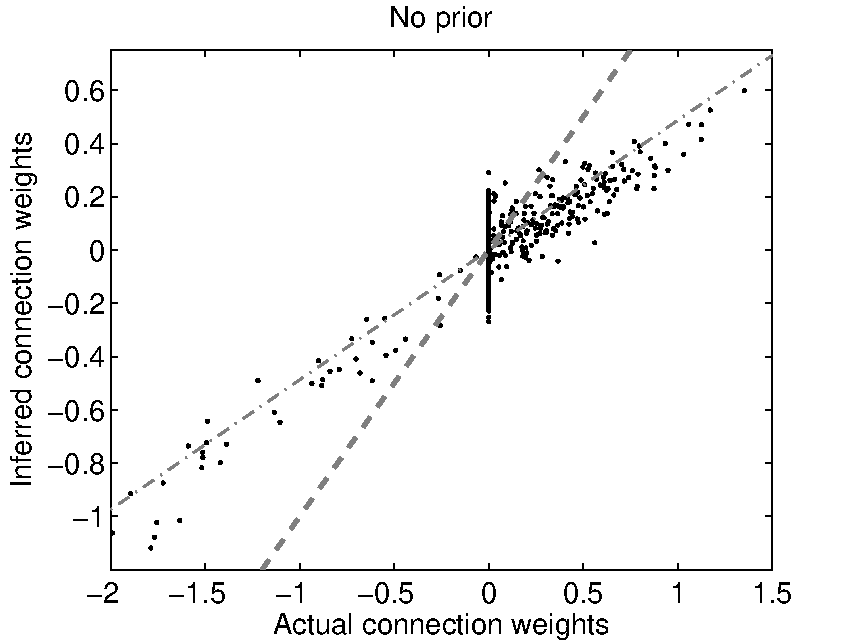
\includegraphics[width=\hsize]{../figs/FigureA10_regular_sol}
\end{minipage}
\begin{minipage}[c]{0.45\hsize}
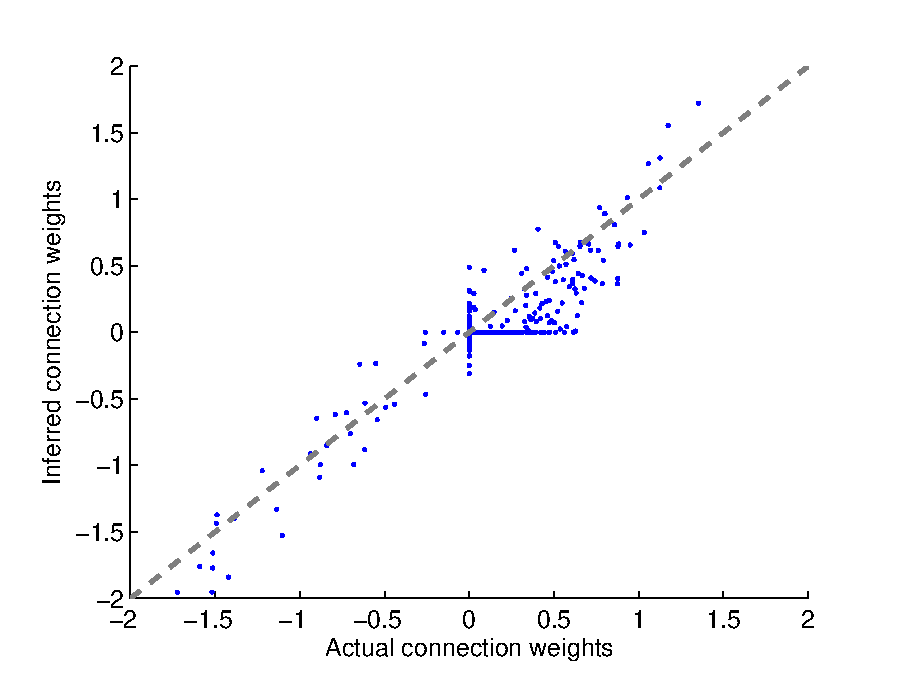
\includegraphics[width=\hsize]{../figs/FigureA10_sparse_sol}
\end{minipage}
\caption{Incorporating simple priors on the distribution of connectivity weights in the Bayesian inference algorithm, such as exponential sparseness prior, is essential to achieve much more accurate reconstructions than using simple GLM from a smaller amount of calcium imaging data. Here, connection weights reconstructed using simple GLM (left panel) or sparse-prior GLM (right panel) are shown in a scatter plot for a network of $N=50$ neurons firing at $\approx 5$ Hz and imaged for $T=600$ sec. $r^2=0.64$ for simple GLM solution and $r^2=0.85$ for sparse-GLM solution.}
\label{fig:sparse}
\end{figure}

\begin{figure}[h]
\centering
\begin{minipage}[c]{0.45\hsize}
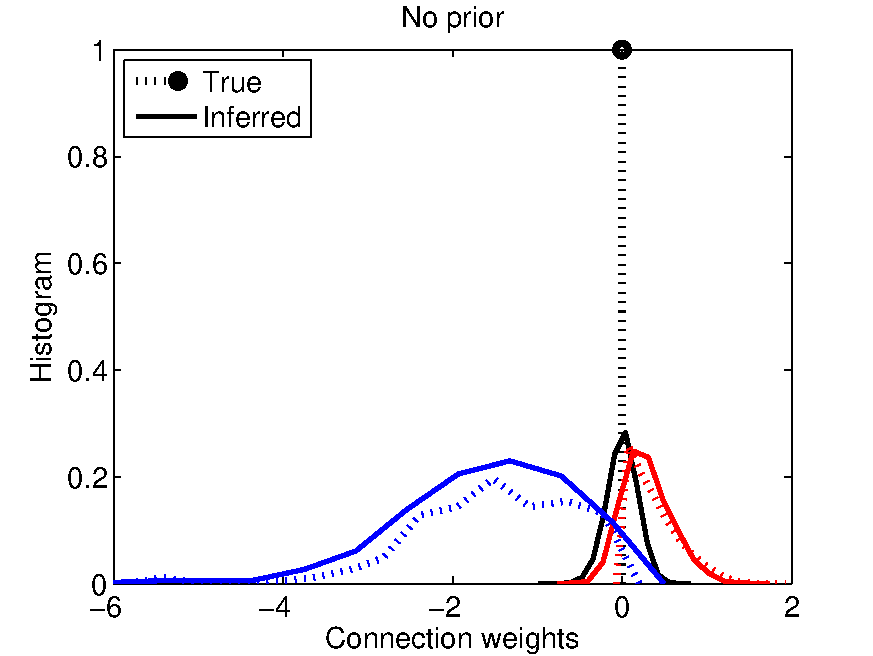
\includegraphics[width=\hsize]{../figs/FigureA3_hist_glm200}
\end{minipage}
\begin{minipage}[c]{0.45\hsize}
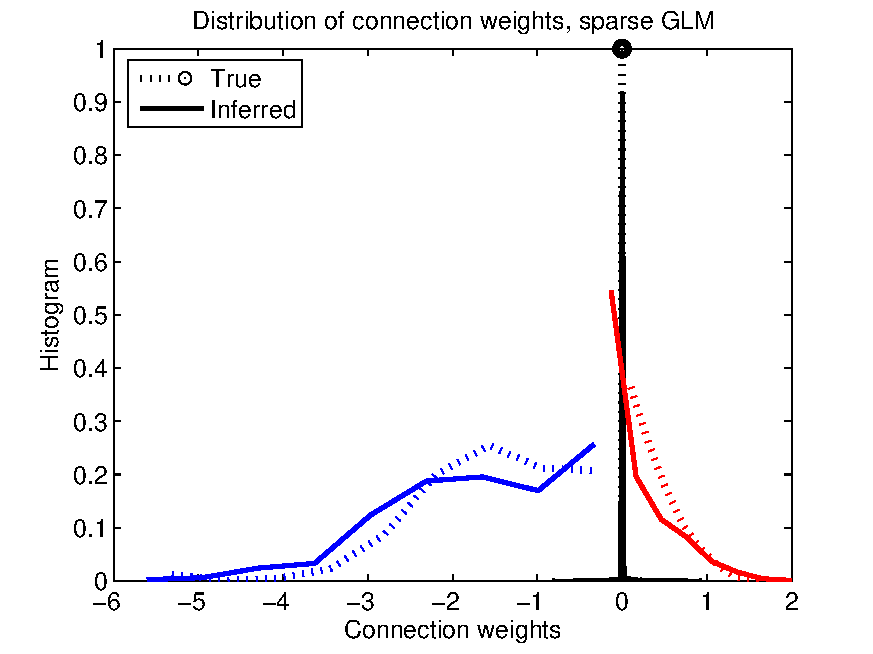
\includegraphics[width=\hsize]{../figs/FigureA3_hist_spa200}
\end{minipage}
\caption{Distribution of inferred connection weights using simple GLM (left) and sparse GLM (right) vs true distributions. When sparse exponential prior on the distribution of connection weights is enacted, dispersion in inferred connection weights is substantially reduced and, in particular, it becomes possible to reliably determine which neural pairs are connected. Distributions are shown for a network of $N=200$ neurons firing at $\approx 5$ Hz and imaged for $T=600$ s was used here.}
\label{fig:distros}
\end{figure}

Taking into account simple prior information about the connectivity matrix resulted in dramatic improvement of the inferred connectivity matrix, Figure \ref{fig:sparse} and \ref{fig:distros}. Sparseness prior resulted in dramatic improvements allowing successful reconstruction from as little as 5 min of calcium imaging data, and allowing to achieve for $T\approx 10$ min the same level of accuracy that would otherwise require up to $T\approx 1$ hour of calcium imaging data, Figure \ref{fig:recvar-NT} and \ref{fig:sparse}.
Note, however, that sparse prior resulted in added scale bias into obtained connectivity estimate, thus, effectively destroying information about the scale of connection weights in a population.
Furthermore, information about connected neural pairs and about inhibitory or excitatory nature of particular neuron could be reliably obtained, Figure \ref{fig:distros}.
Dale's prior, on the other hand, only led to ~10\% in the correlation coefficient $r^2$ of the reconstructed connectivity matrix, and was not found significant.

\subsection{Impact of strong correlations and deviations from generative model on the inference}

%Fig 7: non-robustness to strong correlations
%top panels: rasters
%bottom panels: corrected scatter plots
%
\begin{figure}[h]
\centering
\begin{minipage}[c]{0.45\hsize}
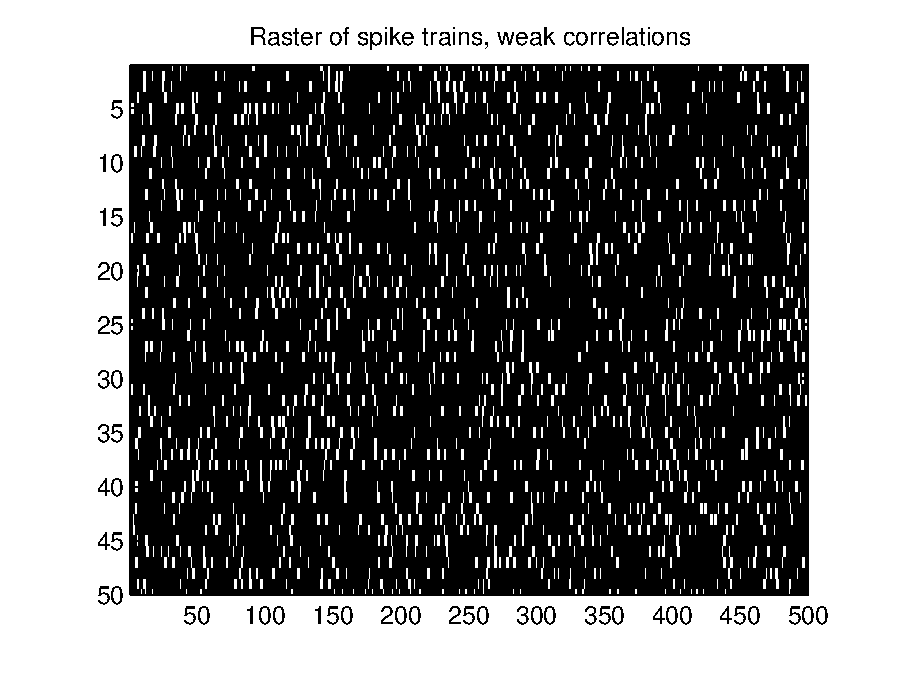
\includegraphics[width=\hsize]{../figs/Figure7b_raster_weak}
\end{minipage}
\begin{minipage}[c]{0.45\hsize}
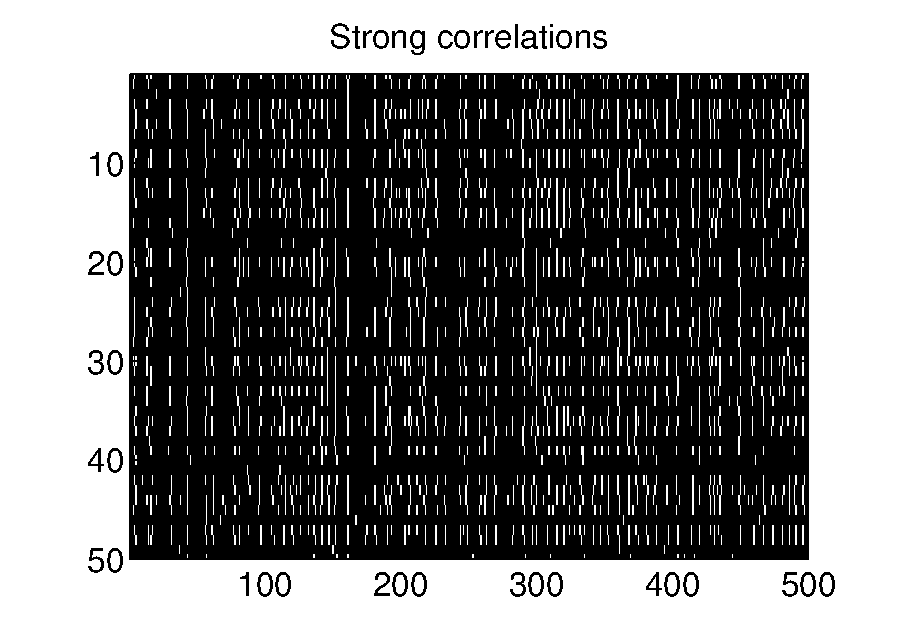
\includegraphics[width=\hsize]{../figs/Figure7a_raster_strong}
\end{minipage}
\begin{minipage}[c]{0.45\hsize}
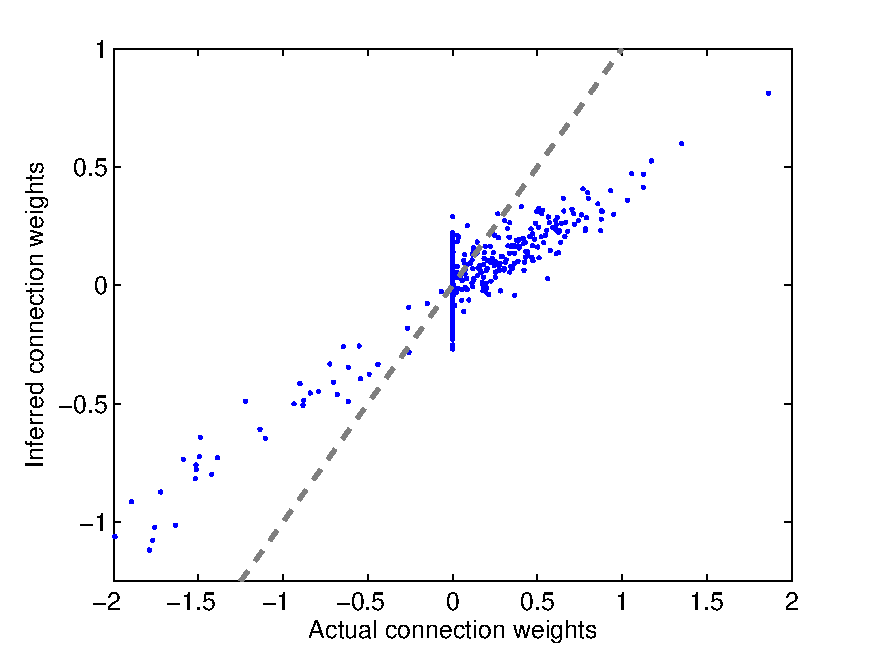
\includegraphics[width=\hsize]{../figs/FigureA8_weak_corr}
\end{minipage}
\begin{minipage}[c]{0.45\hsize}
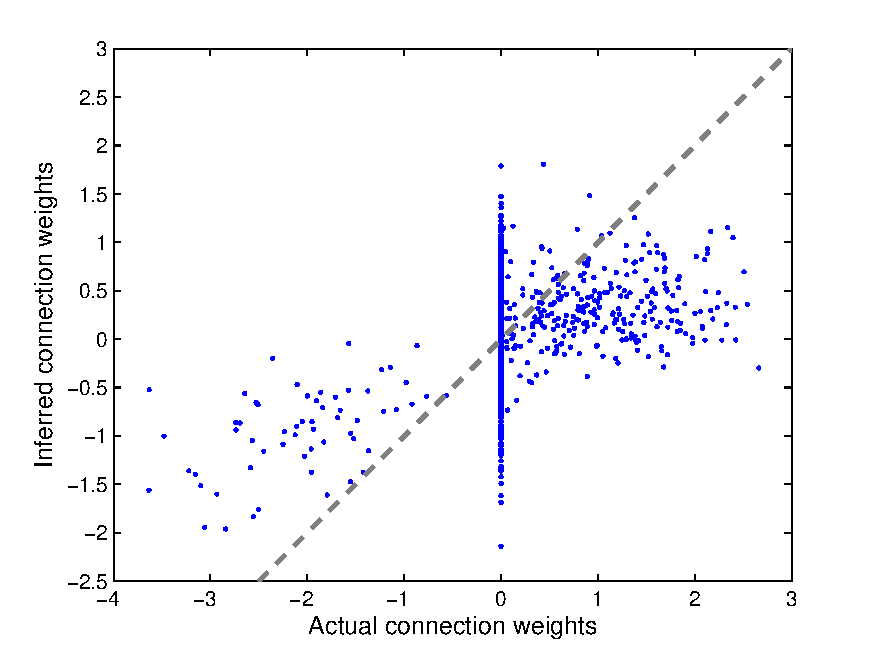
\includegraphics[width=\hsize]{../figs/FigureA8_strong_corr}
\end{minipage}
\caption{
Diverseness of observed neural activity patterns is required for
functional connectivity to give access to the actual ``anatomical'' structure
of the neural circuit. Here, 15 sec of simulated spike trains for a weakly coupled network (upper-left) and a network with strongly coupled component (upper-right) are shown.
In weakly coupled network spikes are sufficiently uncorrelated to give access to all different neural activity patterns needed to properly estimate true weights ${\bf w}_i$. In strongly coupled case, many instances of highly synchronous locked firings are evident, thus preventing observation of sufficiently rich ensemble of activity patterns.
Accordingly, GLM solution for the strongly coupled neural network (lower-right) does not
represent the true connectivity of the circuit, even for the weakly coupled circuit's component. This is contrary to the weakly-coupled network (lower-left) where true connectivity is successfully estimated.
Networks of $N=50$ neurons firing at $\approx 5$ Hz and imaged for $T=600$ sec were used to produce this figure.}
\label{fig:rasters}
\end{figure}

\begin{figure}[h]
\centering
\begin{minipage}[c]{0.45\hsize}
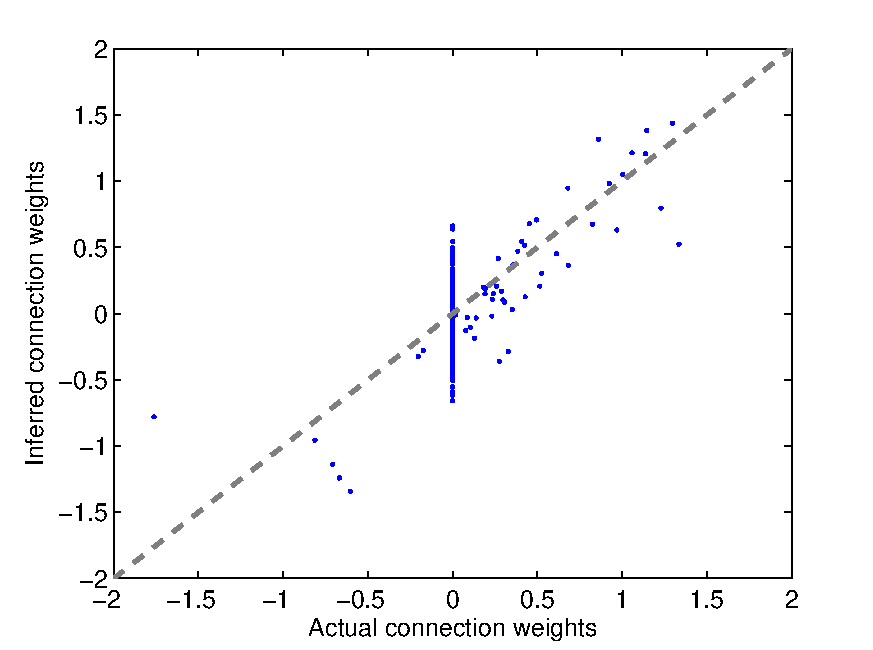
\includegraphics[width=\hsize]{../figs/FigureA9_all_same_sol}
\end{minipage}
\begin{minipage}[c]{0.45\hsize}
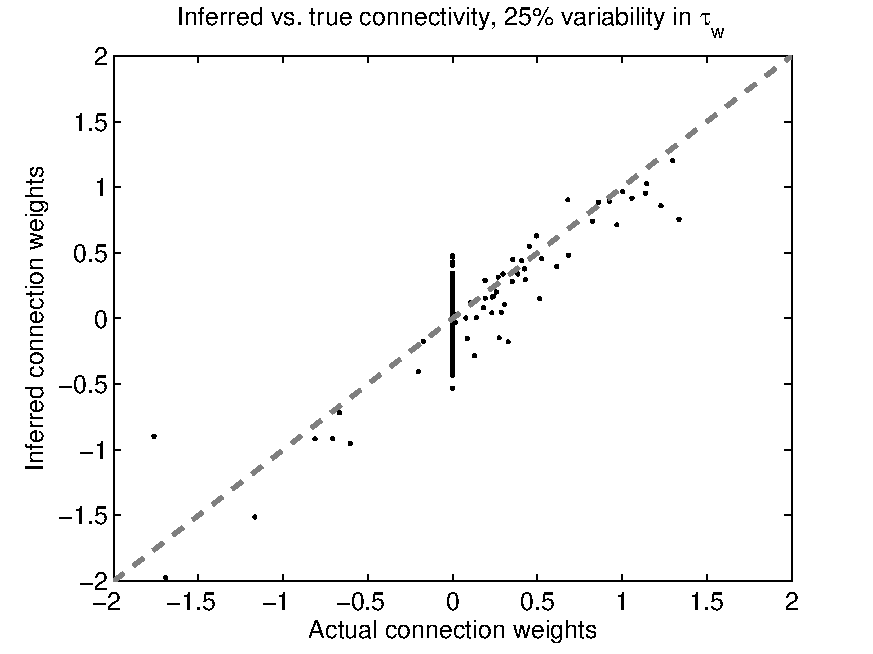
\includegraphics[width=\hsize]{../figs/FigureA9_variable_25}
\end{minipage}
\caption{Bayesian inference algorithm is robust to distortions of the
underlying generative model. One distortion that should be expected is variability of the EPSP time courses from neuron to neuron, and possibly synapse to synapse.
With up to 25\% variability allowed in EPSP time scales $\tau_w$ (right panel) our algorithm provided reconstructions of the same quality as when all $\tau_w$ were the same (left panel). Simulation conditions are the same as in Figure \ref{fig:recvar}.}
\label{fig:vartau}
\end{figure}


``Anatomical'' connectivity was recovered in our experiments despite potential problems noted in the literature [XXX], e.g. such as common input from correlated neurons. This is primarily due to the particular form of the activity in our neural networks, whereas firing of neurons occurred independently, thus, allowing GLM explore the full range of possible input configurations and disentangle common inputs.

Estimation of the functional connectivity is fundamentally routed in observing changes in the spike rate conditioned on the state of the other neurons. Intuitively, such estimation can be compared to observing changes in $p({\bf n}(t))=\exp(\sum_j \w_{ij}n_j(t))$ for different neural configurations ${\bf n}(t)$, i.e. estimating a vector ${\bf w}_i$ from a number of dot-products ${\bf w}_i\cdot {\bf n}(t)$ with different vectors ${\bf n}(t)$. In order to properly estimate all components of ${\bf w}_i$ the set of available ${\bf n}(t)$ should be rich enough to span all $N$ dimensions of ${\bf w}_i$. In case of independent firing such condition is clearly satisfied.  Should this condition be violated, however, e.g. due to high correlation between spiking of few neurons, spike trains may not provide access to the complete vector ${\bf w}_i$, and the connection weights inferred from such activity data may effectively ``aggregate'' true connection weights in arbitrary linear combinations.

We carried out a simulation of hypothetical ``strongly'' coupled  neural network, where in addition to weak sparse connectivity we introduced sparse random strong connectivity component. In some sense, we allowed a fraction of neurons to couple strongly to the other neurons, thus making them ``command'' neurons ``driving'' activity of the other neurons. The strength of strong connectivity component was chosen to build up the actual firing rate dynamically from the baseline rate of $r=\exp(b)\approx 1$ Hz to $\approx 5$  Hz.
Such neural network showed patterns of activity very different from the weakly coupled networks inspected above, Figure \ref{fig:rasters}.  In particular, large number of highly correlated, synchronously locked firings of many neurons were evident in this network.  Likewise, our algorithm was not able to identify the true connectivity matrix correctly, Figure \ref{fig:rasters}.

%Fig 8: robustness to variability in tau_h
%left: corrected scatter plot for (1) assuming same tau's, and (2) assuming they are all diff
%right: distributions of the weights, for truth and the above two approaches
%
%Fig 9: sparse glm improves fit (same format as Fig 8)
%




On the other hand, our inference algorithm showed significant robustness to different deviations from the generative model.
One important deviation that is likely to be present in the real data is variations in the time-scales of EPSPs of different synapses. Up to now, all EPSP time-scales $\tau_w$ were assumed to be the same in our inference algorithm.
Variability in $\tau_w$ would result in added variance in the estimated weights $w_{ij}$ through $\tau_w$ dependence of the scaling factor Eq.(\ref{eqn:bias}).
Still, we found that such added variance to be insignificant in our simulations with $\tau_w$ varying for up to 25\%, Figure \ref{fig:vartau}.


%Fig -: real data
% \begin{figure}[h]
% \centering
% \begin{minipage}[c]{0.45\hsize}
% 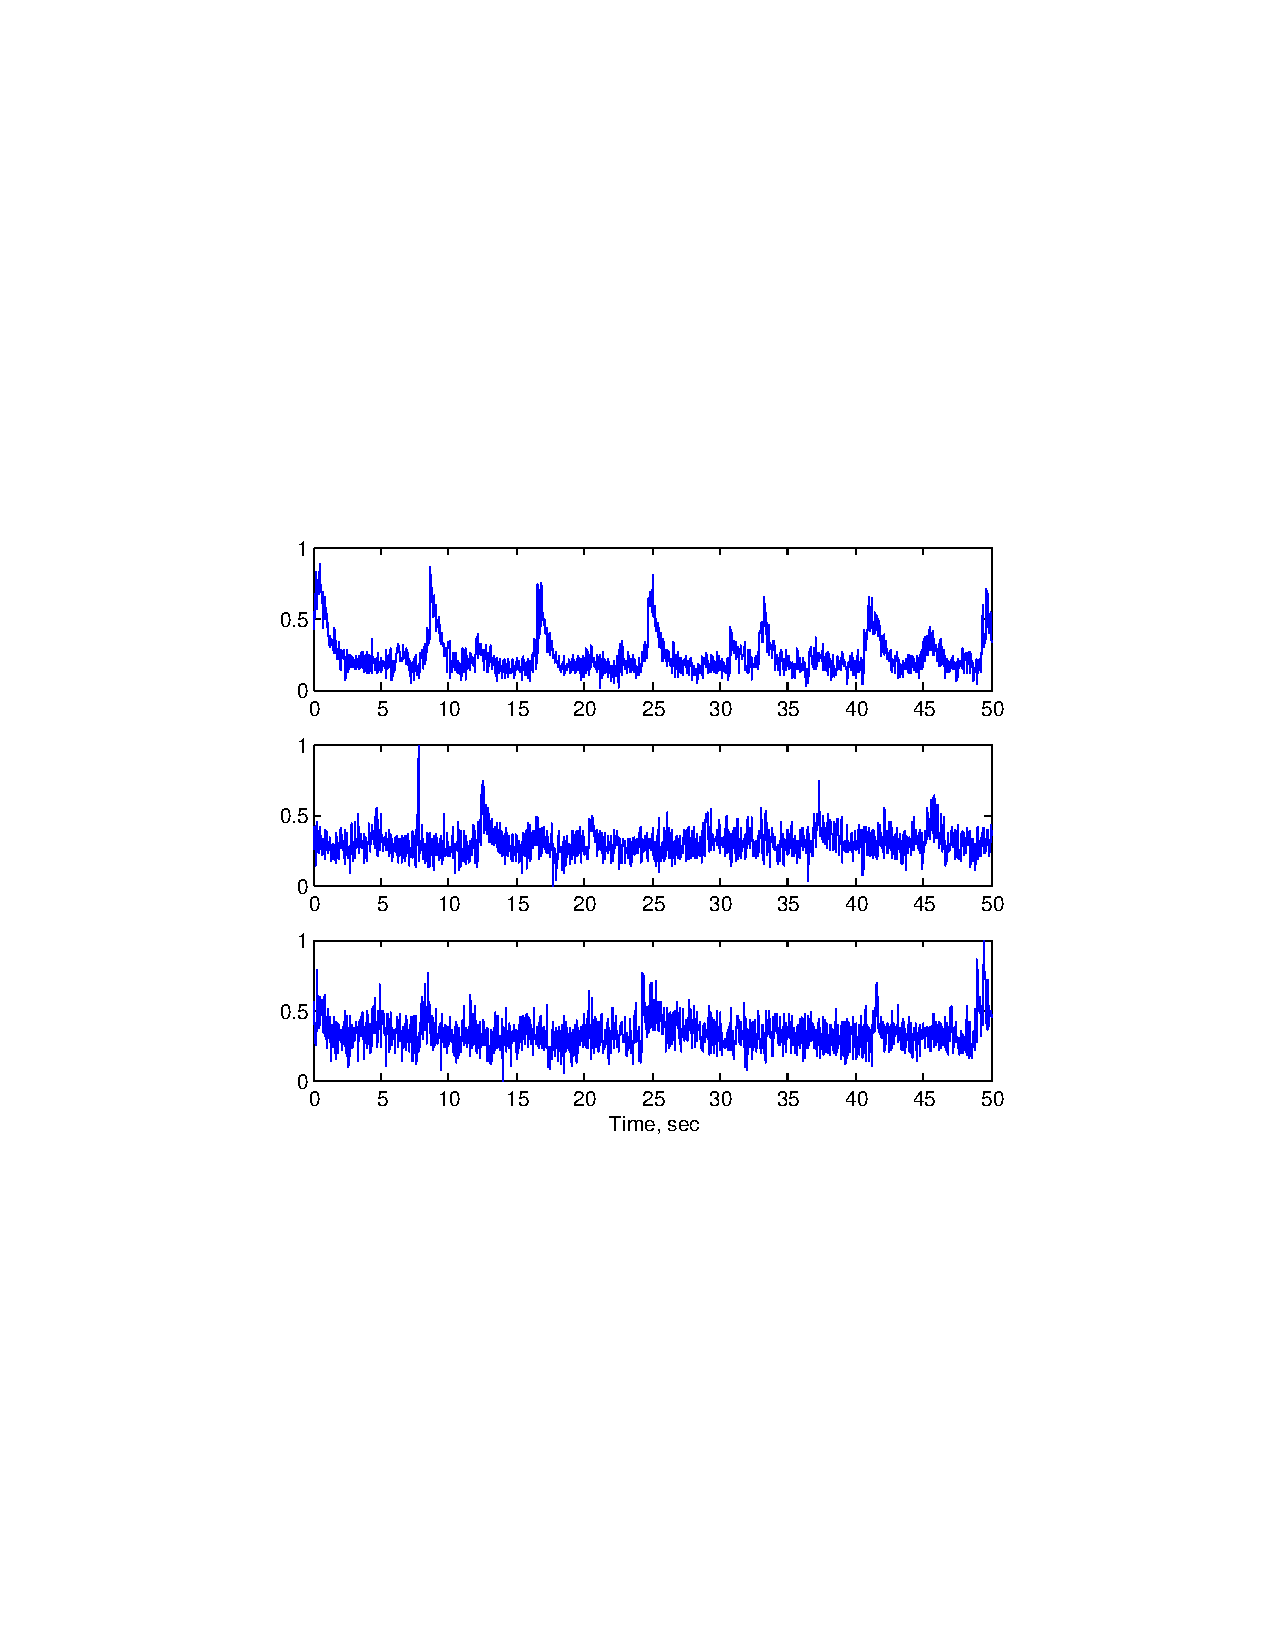
\includegraphics[width=\hsize]{../figs/FigureA11_real_traces}
% \end{minipage}
% \begin{minipage}[c]{0.45\hsize}
% 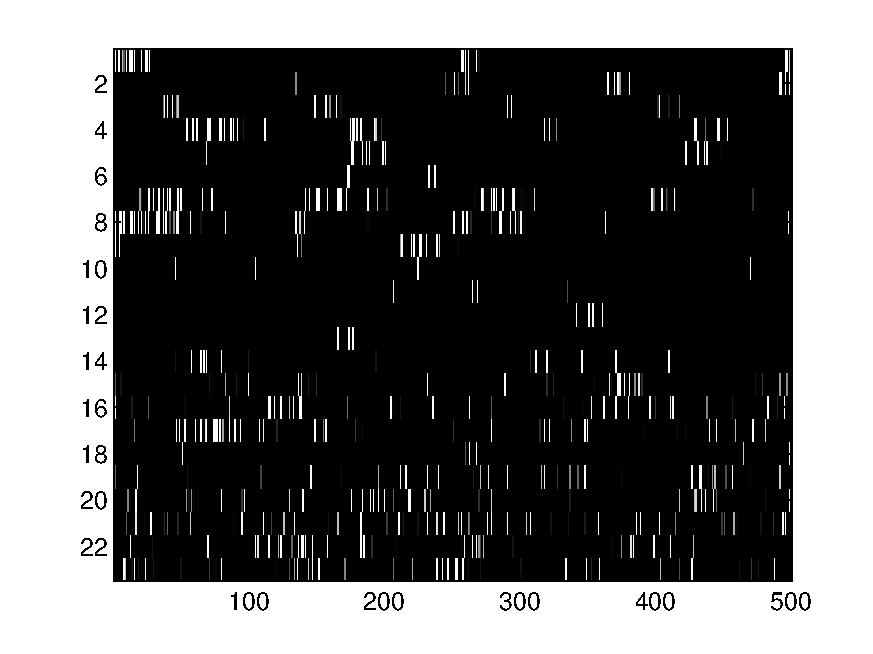
\includegraphics[width=\hsize]{../figs/FigureA11_real_raster}
% \end{minipage}
% \begin{minipage}[c]{0.3\hsize}
% 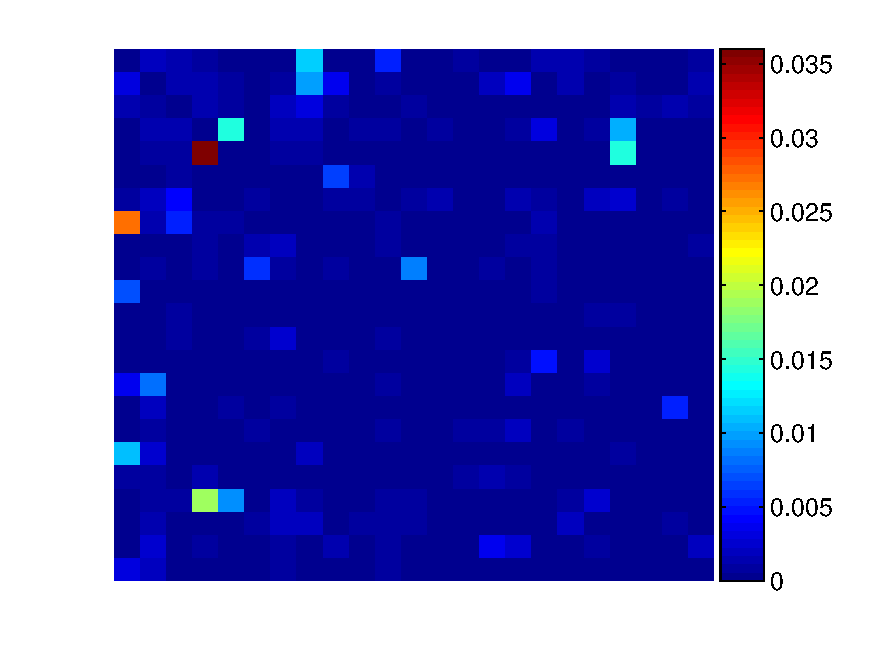
\includegraphics[width=\hsize]{../figs/FigureA11_real_Xcorr}
% \end{minipage}
% \begin{minipage}[c]{0.3\hsize}
% 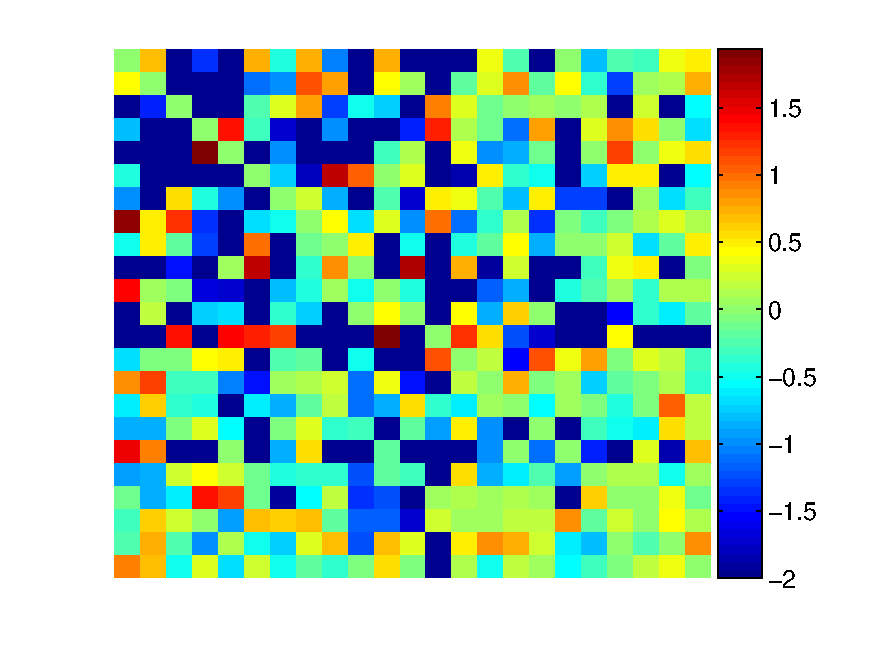
\includegraphics[width=\hsize]{../figs/FigureA11_real_glm}
% \end{minipage}
% \begin{minipage}[c]{0.3\hsize}
% 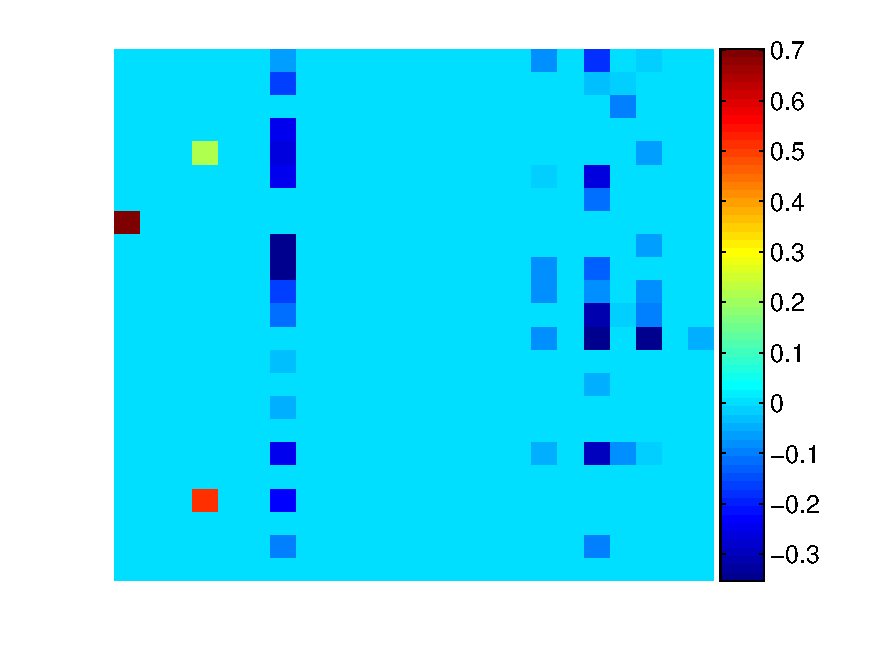
\includegraphics[width=\hsize]{../figs/FigureA11_real_sparse}
% \end{minipage}
% \caption{Functional connectivity matrix inferred from a sample of actual calcium imaging data for $N=72$ cells in [XXX], imaged for $T\approx 260$ sec at 15 Hz.
% $N=23$ neurons with spikes at sufficient SNR were selected, and functional connectivity reconstructed using factorized approximation algorithm. Firing cell of these cells was 0.1-1 Hz and 20-200 spikes were collected for each neuron.
% Upper-left panel shows example of actual fluorescence traces from selected cells, best to worst. Upper-right panel shows a raster of inferred spike trains for first 100 sec of imaging data. Lower panels show left-to-right the time-delayed cross-correlation matrix for selected neurons, simple GLM solution and sparse GLM solution, respectively. A consistent connectivity matrix is obtained here, with sparse solution having sparseness of $\approx 10 \%$, and all neurons automatically respecting Dale's law without explicitly enforcing it. Two clearly excitatory, and three clearly inhibitory neurons can be seen, with remaining neurons not showing significant couplings.}
% \label{fig:real}
% \end{figure}


%We applied our algorithm to a sample of the real calcium imaging data from [XXX], totaling about 5 minutes of imaging for a population of 72 cells in [XXX]. Out of these, about 23 cells had fluorescence traces indicative of spikes, while the other cells were either silent or did not shown SNR sufficient for analysis. These 23 cells were selected for futher processing. 20-200 spikes were found for each cell, corresponding to firing rates from 0.07 Hz to 0.8 Hz.
%We then identified functional connectivity matrix for this population. Sparse solution resulted in consistent connectivity matrix with sparseness of about 10\%, automatically respecting Dale's law, and clearly indicating two strongly connected excitatory neurons and few inihibitory neurons. Although this data lacked independent controls necessary to properly evaluate quality of our obtained reconstruction, it does demonstrate that our approach can be successfully applied under real-life condition to analyze functional connectivity of real populations of neurons.
